

\documentclass[11pt,compress,t,notes=noshow]{beamer}

\usepackage[english]{babel}
\usepackage{dsfont}
\newcommand\bmmax{2}
\usepackage{bm}
\usepackage{bbm}
\usepackage{verbatim}
\usepackage{amsmath}
\usepackage{amsfonts}
\usepackage{csquotes}
\usepackage{multirow}
\usepackage{longtable}
\usepackage{enumerate}
\usepackage[absolute,overlay]{textpos}
\usepackage{psfrag}
\usepackage{algorithm}
\usepackage{algorithmicx}
\usepackage{algpseudocode}
\usepackage{eqnarray}
\usepackage{multimedia}
\usepackage{media9}
\usepackage{arydshln}
\usepackage{tabularx}
\usepackage{placeins}
\usepackage{tikz}
\usepackage{setspace}
\usepackage{wrapfig}
\usepackage{tcolorbox}
\usepackage[export]{adjustbox}
\usepackage{siunitx}
\usetikzlibrary{shapes,arrows,automata,positioning,calc}
\tikzset{
  %Define standard arrow tip
  >=stealth',
  %Define style for boxes
  punkt/.style={
    rectangle,
    rounded corners,
    draw=black, very thick,
    text width=6.5em,
    minimum height=2em,
    text centered},
  % Define arrow style
  pil/.style={
    ->,
    thick,
    shorten <=2pt,
    shorten >=2pt,}
}
\usepackage{subfig}

%new environments

\newenvironment{vbframe}  %frame with breaks and verbatim
{
 \begin{frame}[containsverbatim,allowframebreaks]
}
{
\end{frame}
}

\newenvironment{vframe}  %frame with verbatim without breaks (to avoid numbering one slided frames)
{
 \begin{frame}[containsverbatim]
}
{
\end{frame}
}

\newenvironment{blocki}[1]   % itemize block
{
 \begin{block}{#1}\begin{itemize}
}
{
\end{itemize}\end{block}
}

\newenvironment{fragileframe}[2]{  %fragile frame with framebreaks
\begin{frame}[allowframebreaks, fragile, environment = fragileframe]
\frametitle{#1}
#2}
{\end{frame}}


\newcommand{\myframe}[2]{  %short for frame with framebreaks
\begin{frame}[allowframebreaks]
\frametitle{#1}
#2
\end{frame}}

\newcommand{\remark}[1]{
  \textbf{Remark:} #1
}

%%%%%%%%%%%%%%%%%%%%%%%%%%%%%%%%%%%%%%%%%%%%%%%%%%%%%%%%%%%%%%%%%%%%%%%%%%%%%%%

% basic latex stuff
\newcommand{\pkg}[1]{{\fontseries{b}\selectfont #1}} %fontstyle for R packages
\newcommand{\lz}{\vspace{0.5cm}} %vertical space
\newcommand{\dlz}{\vspace{1cm}} %double vertical space
\newcommand{\oneliner}[1] % Oneliner for important statements
{\begin{block}{}\begin{center}\begin{Large}#1\end{Large}\end{center}\end{block}}


%\usetheme{lmu-lecture}
\usepackage{../style/lmu-lecture}

\let\code=\texttt
\let\proglang=\textsf

\setkeys{Gin}{width=0.9\textwidth}



\title{Deep Learning}
\author{David Rügamer}
\institute{Department of Statistics -- LMU Munich}
\date{Winter Semester 2021}

\setbeamertemplate{frametitle}{\expandafter\uppercase\expandafter\insertframetitle}

%\begin{document}
%\sloppy
%\end{document}


\input{../../latex-math/basic-math}
\input{../../latex-math/basic-ml}
\input{../../latex-math/ml-nn}

\begin{document}

\lecturechapter{2}{Gradient Descent}
\lecture{Deeplearning}

\begin{frame}
\frametitle{Lecture outline}
\tableofcontents
\end{frame}


%%%%%%%%%%%%%%%%%%%%%%%%%%%%%%%%%%%%%%%%%%%%%%%%%%%%%%%%%%%%%%%%%%
\section{Gradient Descent}

%%%%%%%%%%%%%%%%%%%%%%%%%%%%%%%%%%%%%%%%%%%%%%%%%%%%%%%%%%%%%%%%%%
% \begin{vbframe}{Revision: How learning differs from Pure optimization(Remove/Shorten)}
%   \begin{itemize}
%     \item In machine learning we usually act \textbf{indirectly}.
%     \item Technically, we would like to minimize the expected generalization error (or risk):
%       $$\riskt = \E_{(x,y)\sim p_{data}} [\Lxyt]$$
%     with $p_{data}$ being the true underlying distribution.
%     \lz
%       \begin{itemize}
%         \item If we knew $p_{data}$, the minimization of the risk would be an optimization task!
%         \item However, when we only have a set of training samples, we deal with a machine learning problem.
%       \end{itemize}
%   \end{itemize}
% \framebreak
%   \begin{itemize}
%     \item An alternative without directly assuming something about $p_{data}$ is to approximate $\riskt$ based on the training data, by means of the empirical risk:
%       $$\risket = \frac{1}{n} \sumin \Lxyit$$
%     \item So rather than optimizing the risk directly, we optimize the empirical risk, and hope that the risk decreases as well.
%     \item The empirical risk minimization is prone to overfitting as models with high capacity can simply memorize the training set.
%     \item Thus, we have to tweak our optimization such that the quantity that we actually optimize is even more different from the quantity that we truly want to optimize (in reality we obviously optimize $\Oreg$, but to keep things easy we spare that).
%   \end{itemize}
% \end{vbframe}
%%%%%%%%%%%%%%%%%%%%%%%%%%%%%%%%%%%%%%%%%%%%%%%%%%%%%%%%%%%%%%%%%%
% %%%%%%%%%%%%%%%%%%%%%%%%%%%%%%%%%%%%%%%%%%%%%%%%%%%%%%%%%%%%%%%%%%
% \begin{vbframe}{Recall: Gradient descent (Chapter 1)}
%   \begin{center}
%     $f(x_1, x_2) = -\sin(x_1) \cdot \frac{1}{2\pi} \exp\left( (x_2 - \pi / 2)^2 \right)$
% <<echo=FALSE, fig.width=8, fig.height=4>>=
% require("colorspace")
% require("ggplot2")
% foo = function(x, y) {
%   -1 * sin(x) * dnorm(y, mean = pi / 2, sd = 0.8)
% }
% 
% x = y = seq(0, pi, length = 50)
% z = outer(x, y, foo)
% p = c(list(list(.1, 3)), optim0(.1, 3, FUN = foo, maximum = FALSE))
% 
% sd_plot(phi = 25, theta = 20, xlab = "x1", ylab = "x2")
% @
%   \end{center}
%   \hspace{2cm} "Walking down the hill, towards the valley."
% \end{vbframe}
% %%%%%%%%%%%%%%%%%%%%%%%%%%%%%%%%%%%%%%%%%%%%%%%%%%%%%%%%%%%%%%%%%%

%%%%%%%%%%%%%%%%%%%%%%%%%%%%%%%%%%%%%%%%%%%%%%%%%%%%%%%%%%%%%%%%%%
% \begin{vbframe}{Gradient based learning}
%   \begin{itemize}
%     \item Nonlinearity of neural nets causes loss functions to become non-convex. Thus, convex optimization algorithms do not work anymore.
%     \item We use iterative, gradient-based optimization instead!
%     \begin{itemize}
%       \item But: does not guarantee convergence and results may depend heavily on initial parameters.
%     \end{itemize}
%   \end{itemize}
% \end{vbframe}
%%%%%%%%%%%%%%%%%%%%%%%%%%%%%%%%%%%%%%%%%%%%%%%%%%%%%%%%%%%%%%%%%%
%%%%%%%%%%%%%%%%%%%%%%%%%%%%%%%%%%%%%%%%%%%%%%%%%%%%%%%%%%%%%%%%%%
% \begin{vbframe}{Revision of gradient descent}
%   \begin{itemize}
%     \item First we need to recall the method of gradient descent in numerical optimization.
%     \item Let $\fx$ be an arbitrary, differentiable, unrestricted target function, which we want to minimize.
%       \begin{itemize}
%         \item We can calculate the gradient $\nabla \fx$, which always points in the direction of the steepest ascent.
%         \item Thus $-\nabla \fx$ points in the direction of the steepest descent!
%       \end{itemize}
%   \end{itemize}
% \framebreak
%   \begin{itemize}
%     \item Standing at a point $x_k$ during minimization, we can improve this point by doing the following step:
% $$f(x_{k+1}) = f(x_k) - \nu \nabla f(x_k)$$
%  \enquote{Walking down the hill, towards the valley.}
%     \item $\nu$ determined the length of the step and is called step size.
% To find the optimal $\nu$ we need to look at:
% $$g(\nu) = f(x_k) - \nu \nabla f(x_k) = min!$$
%     \item This minimization problem only has one real parameter, and is therefore \enquote{easy} to solve.
% These kind of methods are known as line search methods.
%   \end{itemize}
% \framebreak
%     \begin{figure}
%       \centering
%         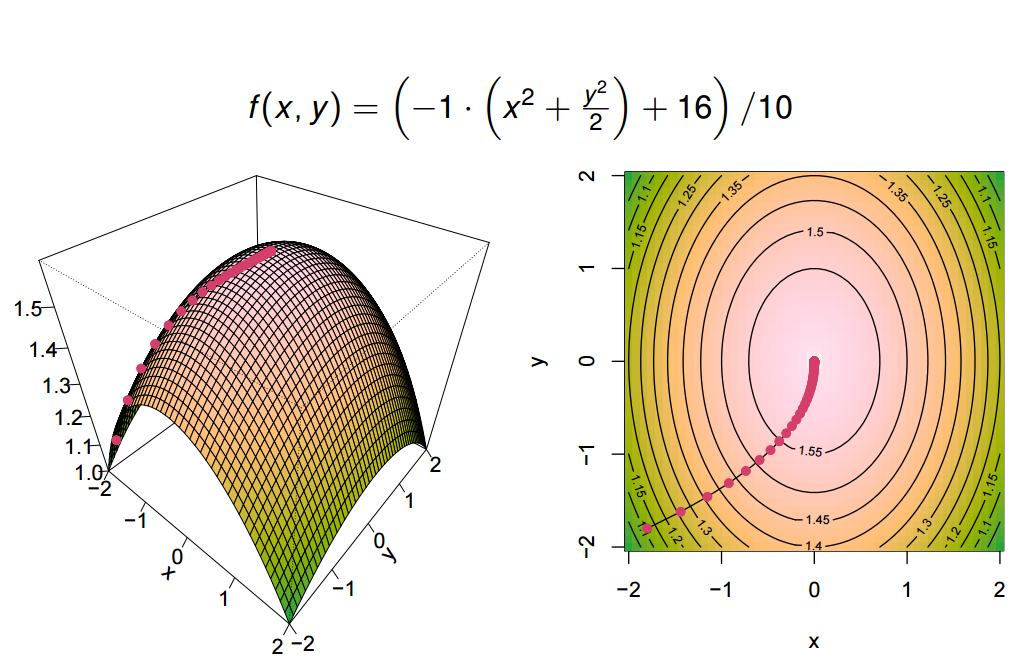
\includegraphics[width=10.2cm]{plots/ascent.png}
%     \end{figure}
% \end{vbframe}
%%%%%%%%%%%%%%%%%%%%%%%%%%%%%%%%%%%%%%%%%%%%%%%%%%%%%%%%%%%%%%%%%%


\begin{vbframe}{Gradient descent}
  \begin{itemize}
    \item Let $\risk: \R^p \to \R$ be an arbitrary, differentiable, unrestricted function (of $\thetab \in \R^p$). \\
    \begin{footnotesize}
    In the context of deep learning, $\risk$ represents the empirical risk function and $\thetab$ represents the weights (and biases) of the network. For simplification, we assume $\bm{\theta} = (\theta_1, ..., \theta_m)$. 
    \end{footnotesize}
    \item We want to minimize this function by gradient descent (GD). 
    \item The negative gradient 
    $$
    - \mathbf{g} = - \nabla \riskt = - \left(\frac{\partial \risk}{\partial \theta_1}, \ldots, \frac{\partial \risk}{\partial \theta_m}\right)^\top
    $$ 
    points in the direction of the \textbf{steepest descent}.
  \end{itemize}

    \framebreak

  \begin{itemize}
    \item \enquote{Standing} at a point $\thetab^{[t]}$ during minimization, we improve by performing the following update: 
    $$
      \thetab^{[t + 1 ]}  = \thetab^{[t]} - \alpha \nabla \risk\left(\thetab^{[t]}\right),
    $$
    which implies (for sufficiently small $\alpha$),
    $$
    \risk(\bm{\thetab}^{[t+1]}) \leq \risk(\bm{\thetab}^{[t]})
    $$
    \item $\alpha$ determines the length of the step and is called \textbf{step size} or, in risk minimization, \textbf{learning rate}.
  \end{itemize}

\end{vbframe} 

\begin{vbframe}{Example: Gradient descent }
  \begin{center}
    $\risk(\theta_1, \theta_2) = -\sin(\theta_1) \cdot \frac{1}{2\pi} \exp\left( (\theta_2 - \pi / 2)^2 \right)$

\begin{center}
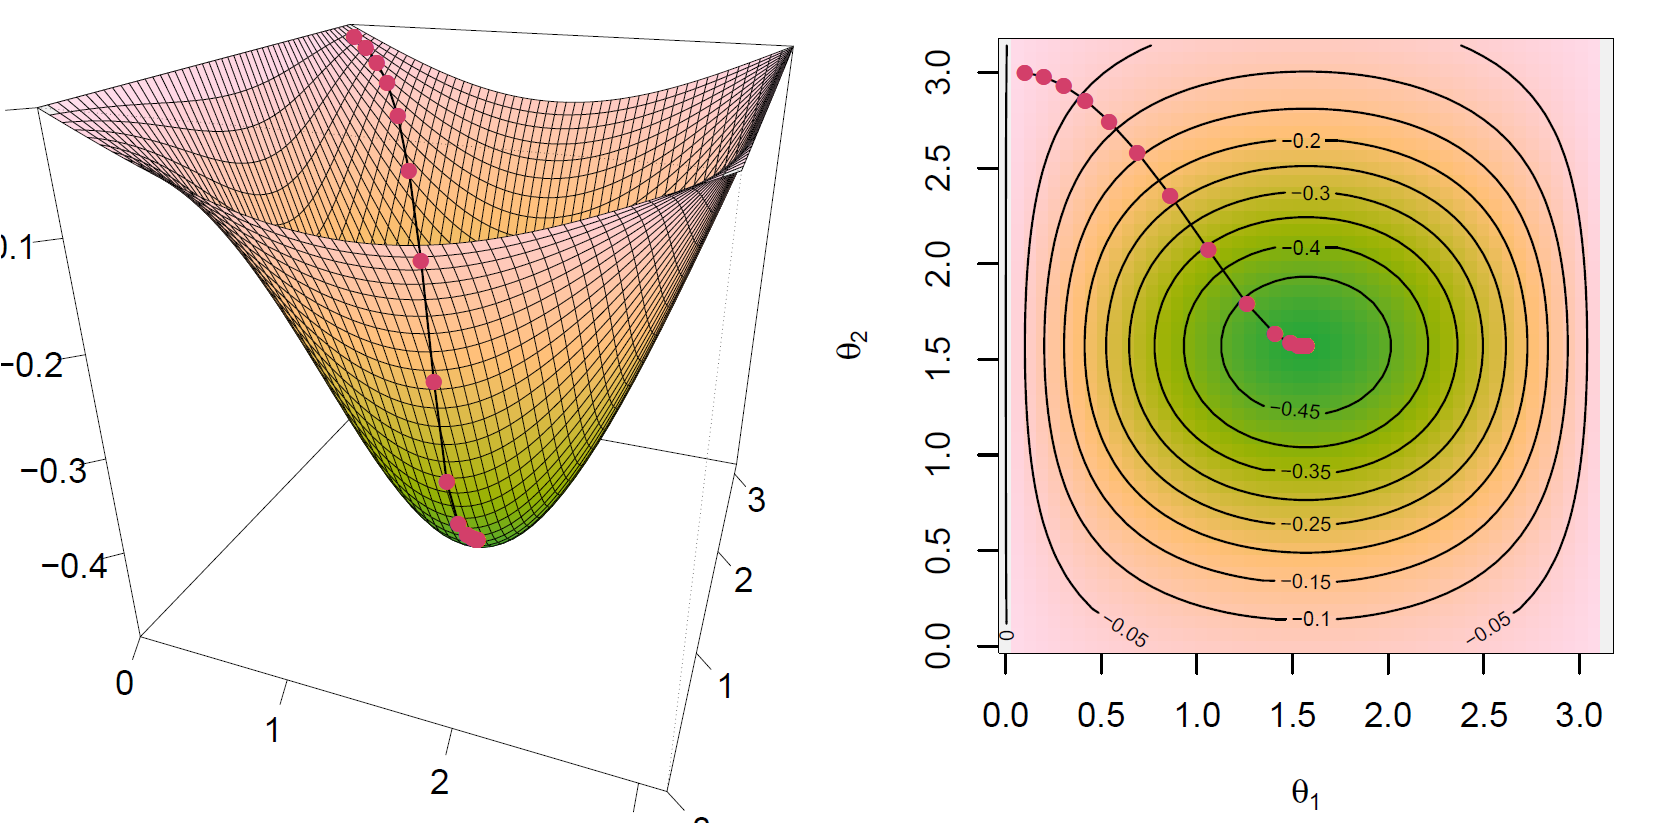
\includegraphics[width=0.9\textwidth]{plots/gradient-descent.png}
\end{center}


  \end{center}
\hspace{2cm} "Walking down the hill, towards the valley."\\
\end{vbframe}

\begin{vbframe}{Gradient Descent and Optimality}

\begin{minipage}{0.45\textwidth}
    \begin{small}
    \begin{itemize}
      \item GD is a greedy algorithm: In every iteration, it makes locally optimal moves.
      \vspace*{2mm}
      \item If $\riskt$ is \textbf{convex} and \textbf{differentiable}, and its gradient is Lipschitz continuous, GD is guaranteed to converge to the global minimum (for small enough step-size).  
      \vspace*{2mm}
    \item However, if $\riskt$ has multiple local optima and/or saddle points, GD might only converge to a stationary point (other than the global optimum), depending on the starting point. 
    \end{itemize}
    \end{small}
  \end{minipage}\hfill
  \begin{minipage}{0.5\textwidth}
    \begin{figure}
      \centering
        \scalebox{1}{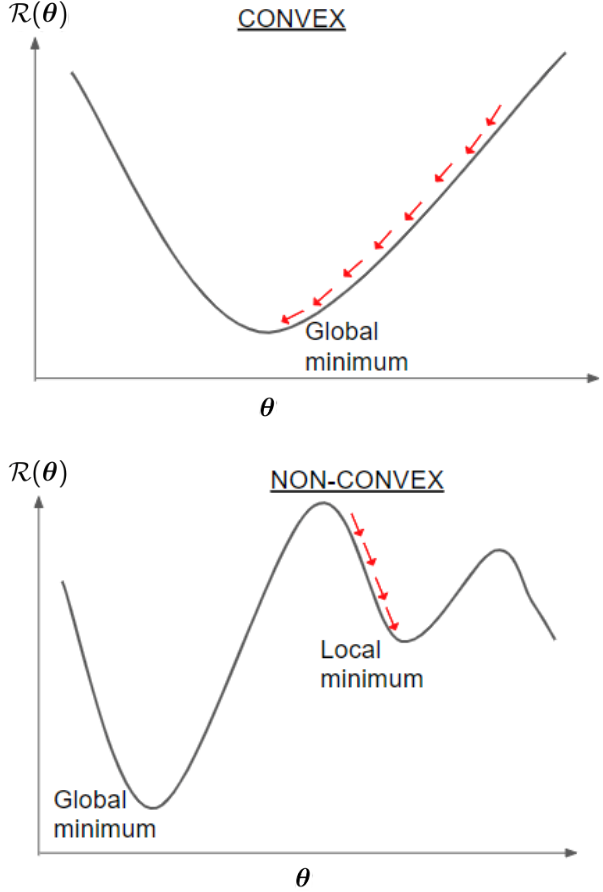
\includegraphics{plots/gdes3.png}}
    \end{figure}
  \end{minipage}  

  \framebreak 

  \textbf{Note: } It might not be that bad if we do not find the global optimum:  

  \begin{itemize}
    \item We do not optimize the actual quantity of interest, i.e. the (theoretical) risk, but only an approximate version, i.e. the empirical risk. 
    \item If the model class is very flexible, it might be disadvantageous to optimize too aggressively and increase the risk of overfitting. 
    \item Early-stopping the optimization might even increase generalization performance. 
  \end{itemize}

\end{vbframe}

%%%%%%%%%%%%%%%%%%%%%%%%%%%%%%%%%%%%%%%%%%%%%%%%%%%%%%%%%%%%%%%%%%


\begin{vbframe}{Learning rate}

The step-size $\alpha$ plays a key role in the convergence of the algorithm.
\lz

If the step size is too small, the training process may converge \textbf{very} slowly (see left image). If the step size is too large, the process may not converge, because it \textbf{jumps} around the optimal point (see right image).

\begin{center}
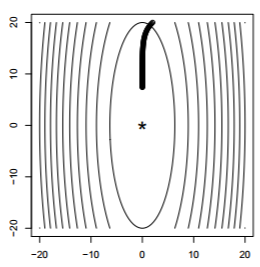
\includegraphics[width = 0.3\textwidth]{plots/stepsize_small.png}~~
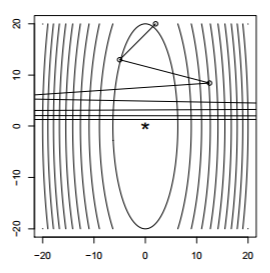
\includegraphics[width = 0.3\textwidth]{plots/stepsize_large.png}
\end{center}

\end{vbframe}

\begin{vbframe}{Learning Rate}


So far we have assumed a fixed value of $\alpha$ in every iteration:

\vspace*{-0.2cm}
$$\alpha^{[t]} = \alpha \quad \forall t = {\{1, \ldots, T\}}$$

% \textbf{Konvergenz:} Es sei $f:\R^n \to \R$ konvex, differenzierbar und Liptschitz-stetig, d.h. es gibt ein $L > 0$
%
% $$
% \|\nabla f(\bm{x}) - \nabla f(\bm{y})\| \le L\|\bm{x} - \bm{y}\| \quad \text{f?r alle} x, y
%

However, it makes sense to adapt $\alpha$ in every iteration:

% We'll look at more sophisticated ways to 

\vspace*{-0.1cm}
\begin{center}
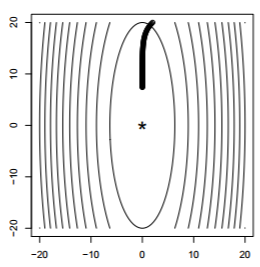
\includegraphics[width = 0.3\textwidth]{plots/stepsize_small.png} ~~~ 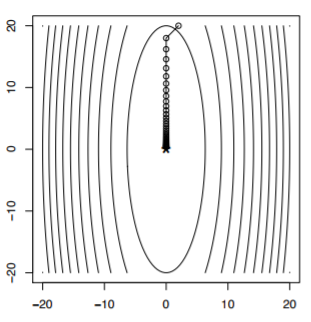
\includegraphics[width = 0.3\textwidth]{plots/stepsize_adaptive.png} \\
\begin{footnotesize}
Steps of gradient descent for $\riskt = 10\,\theta_1^2 + 0.5\,\theta_2^2$. Left:  100 steps for with a fixed learning rate. Right:  40 steps with an adaptive learning rate.
\end{footnotesize}
\end{center}

\end{vbframe}


\section{Stochastic Gradient Descent}


\begin{vbframe}{Stochastic gradient descent}

Let us consider GD for empirical risk minimization. The updates are: 

$$
  \thetab^{[t + 1]} = \thetab^{[t]} - \alpha \cdot \frac{1}{n} \cdot \sumin \nabla_\theta L\left(\yi, f(\xi ~|~ \thetab^{[t]})\right)
$$


  \begin{itemize}
    \item Optimization algorithms that use the entire training set to compute updates in one huge step are called \textbf{batch} or \textbf{deterministic}. This is computationally very costly or often impossible. 
    \item \textbf{Idea:} Instead of letting the sum run over the whole dataset (\textbf{batch mode}) one can also let it run only over small subsets (\textbf{minibatches}), or only over a single example $i$. 
    % \item One \textbf{epoch} means one pass of the full training set.
     \item If the index $i$ of the training example is a random variable with uniform distribution, then its expectation is the batch gradient $\nabla_\theta \risket$
    \item[$\to$] We have a \textbf{stochastic}, noisy version of the batch gradient

    \framebreak 

    \item The gradient w.r.t. a single training observation is fast to compute but not reliable. It can be used simply as a computational trick to deal with large data or to operate on real streams of online data in online learning.
    \item In contrast, the full
    batch gradient is costly (or even impossible, e.g., when data does not even fit into memory) to compute, particularly in DL, but it averages out all the noise from sub-sampling.
    \item Minibatches are in between. The batch size decides upon the compromise
    between speed and averaging (smoothing).
    \item In summary: SGD computes an unbiased estimate of the gradient by taking the average gradient over a minibatch (or one sample) to update the parameter $\thetab$ in this direction.
    % \item Optimization algorithms that use only a single example at a time are called \textbf{stochastic} or \textbf{online}. This can be used simply as a computational trick to deal with large data or to operate on real streams of online data in online learning.
% Those methods are called \textbf{minibatch} or \textbf{stochastic}.
  \end{itemize}
 

  \framebreak
 
 An illustration of the SGD algorithm (to minimize the function $1.25(x_1 + 6)^2 + (x_2 - 8)^2)$.
 \begin{figure}
    \scalebox{0.8}{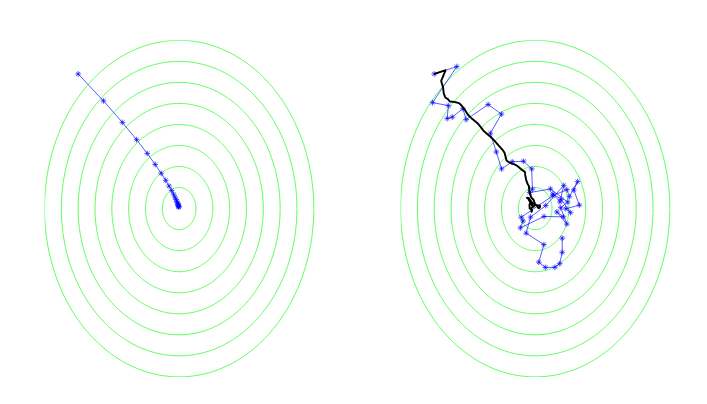
\includegraphics{SGD.png}}
    \tiny{\\ source : Shalev-Shwartz and  Ben-David.
Understanding machine learning: From theory to algorithms. Cambridge University Press, 2014. }
 \caption{On the left is GD and on the right is SGD. The black line depicts the averaged value of $\thetab$.}
 \end{figure}
 

  \framebreak
  
  % \begin{algorithm}[H]
  % \footnotesize
  %   \caption{Basic SGD pseudo code}
  %   \begin{algorithmic}[1]
  %   \State Initialize parameter vector $\thetab^{[0]}$ 
  %   \State Randomly shuffle data and partition into minibatches $J_1, ..., J_k$ of size $m$
  %   \State $t \leftarrow 0$
  %   \While{stopping criterion not met}
  %   \State Take a minibatch $J$ of $m$ examples from training set, $J \subset \nset$
  %       \State Compute gradient estimate: $\hat{g}^{[t]} \leftarrow \frac{1}{m} \sum_{i \in J} \nabla_\theta L(\yi, f(\xi ~|~ \thetab^{[t]}) $
  %       \State Apply update: $\thetab^{[t]} \leftarrow \thetab^{[t-1]} - \alpha \hat{g}^{[t]}$
  %       \State $t \leftarrow t + 1$
  %     \EndWhile
  %   \end{algorithmic}
  % \end{algorithm}
  % \begin{itemize}
  %   \item Thus, what SGD basically does is computing an unbiased estimate of the gradient by taking the average gradients of a minibatch to update the parameter $\thetab$.
  % \end{itemize}
  
%\framebreak

  \begin{algorithm}[H]
  \footnotesize
    \caption{Basic SGD pseudo code}
    \begin{algorithmic}[1]
    \State Initialize parameter vector $\thetab^{[0]}$ 
    
    \State $t \leftarrow 0$
    \While{stopping criterion not met}
    \State Randomly shuffle data and partition into minibatches $J_1, ..., J_K$ of size $m$
      \For{$k\in\{1,...,K\}$} 
      \State $t \leftarrow t + 1$ 
      \State Compute gradient estimate with $J_k$: $\hat{g}^{[t]} \leftarrow \frac{1}{m} \sum_{i \in J_k} \nabla_\theta L(\yi, f(\xi ~|~ \thetab^{[t-1]})) $
      \State Apply update: $\thetab^{[t]} \leftarrow \thetab^{[t-1]} - \alpha \hat{g}^{[t]}$
      
      \EndFor
    
        
      \EndWhile
    \end{algorithmic}
  \end{algorithm}
  % \begin{itemize}
  %   \item Thus, what SGD basically does is computing an unbiased estimate of the gradient by taking the average gradients of a minibatch to update the parameter $\thetab$.
  % \end{itemize}
  
\framebreak

\vspace*{0.5cm}
  \begin{itemize}
    \item With minibatches of size $m$, a full pass over the training set (called an \textbf{epoch}) consists of $\frac{n}{m}$ gradient updates.
    \item SGD and its modifications are the most used optimization algorithms for ML in general and for deep learning in particular.
    \item SGD (with one or a few samples per batch) updates have a high variance, even though they are unbiased. 
      Because of this variance, the learning rate $\alpha$ is typically much smaller than in the full-batch scenario.

\framebreak 

\vspace*{0.5cm}

    \item When the learning rate is slowly decreased, SGD converges to a local minimum.
    \item SGD with minibatches reduces the variance of the parameter updates and utilizes highly optimized matrix operations to efficiently compute gradients.
    \item Minibatch sizes are typically between 50 and 1000.
    \item Recent results indicate, that SGD often leads to better generalizing models then GD, and thus may perform some kind of indirect regularization.
  \end{itemize}
\end{vbframe}

%%%%%%%%%%%%%%%%%%%%%%%%%%%%%%%%%%%%%%%%%%%%%%%%%%%%%%%%%%%%%%%%%%
%%%%%%%%%%%%%%%%%%%%%%%%%%%%%%%%%%%%%%%%%%%%%%%%%%%%%%%%%%%%%%%%%%
%%%%%%%%%%%%%%%%%%          REFERENCES          %%%%%%%%%%%%%%%%%%
%%%%%%%%%%%%%%%%%%%%%%%%%%%%%%%%%%%%%%%%%%%%%%%%%%%%%%%%%%%%%%%%%%

%\section{References}

\begin{vbframe}
\frametitle{References}
\footnotesize{
\begin{thebibliography}{99}

%%%%%%%%%%%%%%%%%%%%%%%%%%%%%%%%%%
\bibitem[Sebastian Ruder, 2017]{1} Sebastian Ruder (2017)
\newblock An overview of gradient descent optimization algorithms
\newblock \emph{\url{https://arxiv.org/pdf/1609.04747.pdf}}
%%%%%%%%%%%%%%%%%%%%%%%%%%%%%%%%%%

\end{thebibliography}
}
\end{vbframe}
%%%%%%%%%%%%%%%%%%%%%%%%%%%%%%%%%%%%%%%%%%%%%%%%%%%%%%%%%%%%%%%%%%
%%%%%%%%%%%%%%%%%%%%%%%%%%%%%%%%%%%%%%%%%%%%%%%%%%%%%%%%%%%%%%%%%%

\endlecture
\end{document}